\documentclass[14pt]{matmex-diploma-custom}


\usepackage{fontspec}                % font for emoji
\newfontfamily\DejaSans{DejaVu Sans}


\usepackage[section]{placeins}
\usepackage{booktabs}       % professional-quality tables
\usepackage{cleveref}       % reference section with capital letter
\usepackage{natbib}
\usepackage{caption}        % table caption margin
\usepackage{subcaption}     % images next to each other
\usepackage{graphicx}





\begin{document}

\filltitle{ru}{
	chair              = {Математическое обеспечение и администрирование информационных систем\\Кафедра информационно-аналитических систем},
	title              = {Построение гибридной рекомендательной системы новостей с применением методов оптимизации},
	type               = {diploma},
	position           = {студента},
	group              = 441,
	author             = {Смирнов Александр Львович},
	supervisorPosition = {к.ф.-м.н., доц.},
	supervisor         = {Михайлова Елена Георгиевна},
	reviewerPosition   = {руководитель отдела инженерии},
    reviewer           = {Осипов Е.В.}
    
}

\filltitle{en}{
	chair              = {Software and Administration of Information Systems\\Department of Information and Analytical Systems},
	title              = {A Hybrid Approach for News Recommender System using Optimization Methods},
	type               = {diploma},
	position           = {student},
	group              = 441,
	author             = {Alexander Smirnov},
	supervisorPosition = {professor},
	supervisor         = {Elena Mikhaylova},
	reviewerPosition   = {head of engineering department},
    reviewer           = {Evgenii Osipov},
}

\maketitle

\tableofcontents

\section{Введение}

Рекомендательная система является важной частью каждого приложения, в котором содержится большое количество контента и действий пользователей. Огромный объем информации приводит к тому, что пользователь не может найти релевантный для себя контент.

    Рекомендательные системы были испольюзуются для рекомендаций фильмов, музыки и книг \citep{movies} \citep{films} \citep{books}. Рекомендательной системой называется любая система, которая выдает персонализированные рекомендации или направляет пользователя к интересным или полезным объектам в большом пространстве возможных вариантов. Такие системы имеют очевидное преимущество в среде, где объем информации значительно превосходит возможности человека ее исследовать.

    Системы рекомендаций теперь являются неотъемлемой частью некоторых сайтов электронной коммерции, таких как Amazon.com и CDNow \citep{commerce}. Критерии «индивидуальности» и «интересности и полезности», отделяют рекомендательную систему от информационно-поисковых систем \citep{coin}. Семантика поисковой системы - «соответствие»: система должна возвращать все те элементы, которые соответствуют запросу, ранжированные по степени релевантности. Такие методы, как обратная связь по релевантности, позволяют поисковой системе уточнить представление запроса пользователя и представляют собой простую форму рекомендации.

    Сфера рекомендаций новостей имеет свою специфику: новости быстро стареют и это нужно учитывать.

     Существует три основных типа рекомендаций: на основе памяти, на основе модели и гибридные \citep{survey}. Методы на основе памяти \citep{memory} обычно используют метрики сходства для определения расстояния между двумя пользователями или двумя элементами. Методы, основанные на моделях, используют демографическую, информационную или агрегированную информацию для создания модели, которая генерирует рекомендации. Гибридные методы \citep{combining} комбинируют различные типы рекомендателей для повышения качества рекомендаций.

    Общие подходы, такие как коллаборативная фильтрация, имеют свои проблемы: холодный старт, масштабируемость и разреженность данных. Контентные подходы страдают от того факта, что мы должны каким-то образом представлять рекомендуемый элемент в пространстве признаков.

    В этой статье описана гибридная рекомендательная система.
    
    Для единообразия в ходе работы мы перечисляем некоторые термины с их значениями:

        \begin{itemize}
            \item Рейтинг: скалярное значение, отражающее степень релевантности
                \begin {itemize}
                    \item явный (напрямую от пользователя, например, фильм с рейтингом пользователей)
                    \item неявный (выводится из активности пользователя, например, пользователь перестал смотреть фильм через 5 минут)
                \end {itemize}
            \item Прогноз: оценка рейтинга
            \item Рекомендация: выбранные ранжированные элементы для пользователя
            \item Содержимое: атрибуты, текст и т. д .; все о рекомендуемом предмете
        \end {itemize}


    Остальная часть диплома организована следующим образом:
    
        \begin {itemize}
            \item \Cref{sec:related} описывает связанные работы
            \item \Cref{sec:overview} содержит обзор нашего подхода
            \item \Cref{sec:input} описывает входные данные
            \item \Cref{sec:approach} объясняет наш подход
            % \ item \ Cref {sec: implementation} описывает реализацию алгоритмов в реальной системе.
            \item \Cref{sec:evaluation} предоставляет тесты и эксперименты, подтверждающие
результаты нашей системы
            \item \Cref{sec:summary} представляет выводы
        \end {itemize}




\section {Связанные работы}
\label {sec:related}

Согласно исследованию \citep {progress}, методы глубокого обучения не должны превосходить концептуально и вычислительно более простые алгоритмы, поэтому мы не будем их рассматривать.

Наша цель - выбрать оптимальный алгоритм для каждой из следующих задач, чтобы впоследствии комбинировать их:

\begin {itemize}
    \item \textbf {Коллаборативная фильтрация}: создание прогнозов об интересах пользователя путем сбора информации о предпочтениях или вкусовых предпочтениях других пользователей. Он основан на предположении, что если человек A придерживается того же мнения, что и человек B, по какой-либо проблеме, A с большей вероятностью будет иметь мнение B по другому вопросу, чем мнение случайно выбранного человека; по этой теме было проведено много исследований, но статья \citep{evaluation} доказывает, что хорошо настроенный базовый подход SVD ++ превосходит недавно представленные алгоритмы глубокого обучения.
    \item \textbf {Фильтрация на основе содержимого}: основана на предположении, что людям, которым нравились новости с определенными содержимым в прошлом, понравятся такие же элементы и в будущем. Из истории собирается профиль предпочтений пользователя, который впоследствии сравнивается с кандидатами на рекомендации.
    \item \textbf {Фильтрация на основе текущей сессии}: рекомендует на основе активности пользователя в текущем сеансе.
    \item \textbf {Фильтрация по популярности}: использует такую информацию, как количество просмотров, показов, комментариев и т. д.
    \item \textbf {Демографическая фильтрация}: использует демографические данные, такие как возраст, пол, образование и т. д., для определения категорий пользователей.
    \item \textbf {Фильтрация на основе времени}: это способ, при котором более свежие элементы получают более высокие оценки
\end {itemize}

Также есть несколько способов \citep {survey1} комбинировать рекомендатели между собой:

\begin {itemize}
    \item \textbf {Взвешено}: оценки (или голоса) нескольких методов рекомендаций объединяются для получения единой рекомендации.
    \item \textbf {Переключаясь}: система переключается между методами рекомендаций в зависимости от текущей ситуации.
    \item \textbf {Смешанный}: рекомендации от нескольких разных рекомендателей отображаются одновременно.
    \item \textbf {Комбинированный}: функции из разных источников рекомендаций объединены в единый алгоритм рекомендаций.
    \item \textbf {Стекинг}: выходные данные одного метода используются как входные данные для другого.

\end {itemize}


Мы сталкиваемся с проблемой, что миллионы новостей теоретически подходят для рекомендации, поэтому использовать вышеупомянутые методы на таком большом массиве данных некорректно. Вместо этого, как указано в статье \citep {youtube}, мы хотим реализовать конвейер \texttt {генерация кандидатов} $ \to $ \texttt {ранжирование}, чтобы уменьшить количество кандидатов.



\section{Обзор решения}
\label{sec:overview}

Нашей задачей является скомбинировать лучшие подходы в области рекомендательных систем.
Решение состоит из двух частей:

\begin{itemize}
    \item \textbf{Генерация кандидатов}: уменьшение количества рекомендуемых новостей. Эти кандидаты предназначены для фильтрации совсем не релевантного (напр., устаревшего) контента.
    \item \textbf{Ранжирование}: применяем лучшие в своей области алгоритмы для ранжирования оставшихся новостей
\end{itemize}

Архитектура представлена на Рис \cref{fig:architecture}:

\begin{figure}[h]
    \centering
    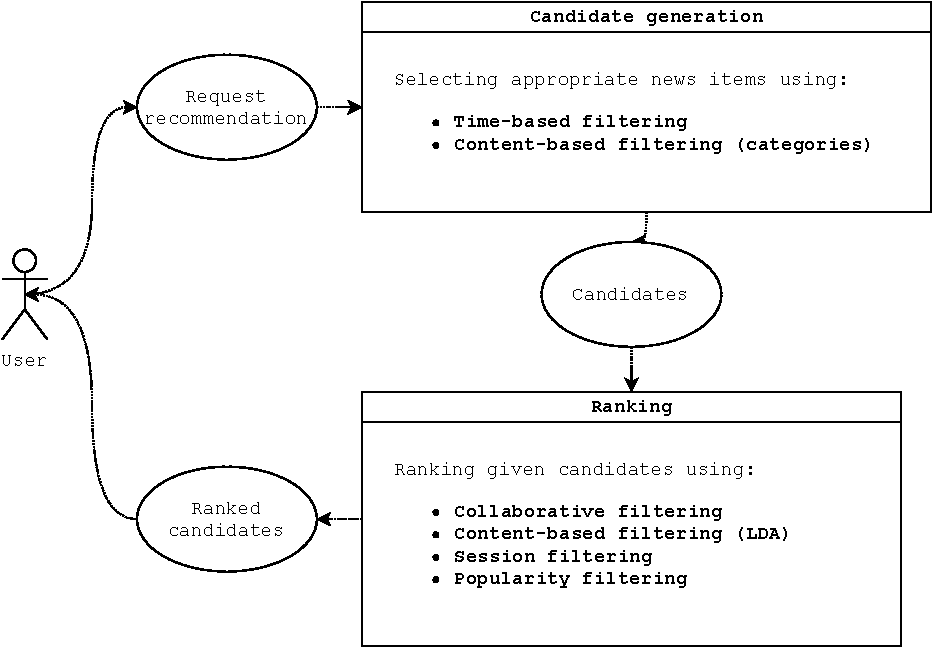
\includegraphics[width=0.8\textwidth]{./images/architechture.pdf}
    \caption{архитектура}
    \label{fig:architecture}
\end{figure}

\section{Входные данные}
\label{sec:input}

Поскольку мы решаем предметную задачу, у нас есть данные о предметной области.
Наши данные состоят из информации о новостях и включают в себя следующие таблицы:

\subsection*{метаданные}

Метаданные о новостях. Здесь у нас есть столбец \textit {item\_id}, который обозначает уникальный идентификатор элемента, затем \textit{date}, который показывает, когда этот элемент был выпущен. Столбец \textit {source\_id} обозначает идентификатор издателя этой новости. Столбец \textit {category} означает категорию текущей новости. Эта категория берется из текста новости по ключевым словам.


\begin{table}[h]
    \centering
    % \resizebox{\textwidth}{!}{
    \begin{tabular}{ccccc}
        \toprule

        \emph{item\_id} & \emph{date} & \emph{source\_id} & \emph{category}\\\midrule

        1 & 2021-01-08 22:08:39 & 9  & politics, conflicts\\
        2 & 2021-01-09 10:28:58 & 5  & IT, social media\\
        3 & 2021-01-09 14:20:34 & 12 & accident\\
        \vdots & \vdots & \vdots & \vdots \\\bottomrule
    \end{tabular}
    % }

    \caption{метаданные}
    \label{tab:meta}
\end{table}


% \begin{itemize}
%     \item \emph{source\_id}: source of news item
% \end{itemize}


\subsection*{содержимое}

В таблице содержимого содержатся тексты новостей в столбце \\
\textit {news\_content}. Это основная информация, которая используется нашей системой рекомендаций, потому что мы можем извлекать много ценных данных из текста, такие как темы.

\begin{table}[h]
    \centering
    \resizebox{\textwidth}{!}{
    \begin{tabular}{cll}    \toprule

        \emph{item\_id} &  \emph{news title} & \emph{news content} \\\midrule

    1  &  Azerbaijan denies reports on construction of Turkish air bases in the country & Information that Turkey will create air bases ...        \\
    2  &  Durov announced the massive transition of WhatsApp users to Telegram          & Telegram developer Pavel Durov said in his channel ...   \\
    3  &  Passenger plane that disappeared from radar crashed                           & Passenger plane taking off from Jakarta, disappeared ... \\
    \vdots & \vdots & \vdots \\\bottomrule
    \end{tabular}
    }
    \caption{содержимое}
    \label{tab:item}
\end{table}

\subsection*{показы \& просмотры}

Поскольку мы работаем с действиями пользователей, у нас должны быть журналы логов, например, какие элементы были нажаты и в какое время, поэтому у нас есть отдельная таблица, содержащая эту информацию. \emph {shows} означает, что \emph {item\_id} был показан \emph {user\_id}, \emph {views} - если \emph {item\_id} был нажат пользователем \emph {user\_id }.

\begin{table}[h]
    \parbox{.45\textwidth}{
        \centering
        \begin{tabular}{ccc}
            \toprule

            \emph{user\_id} & \emph{item\_id} \\\midrule
            10 & 1  \\
            10 & 2  \\
            23 & 1  \\
            23 & 3  \\
            23 & 2  \\
            38 & 3  \\
            38 & 1  \\
            \vdots & \vdots  \\\bottomrule
        \end{tabular}
        \caption{показы}
        \label{tab:show}
    }
    \hfill
    \parbox{.45\textwidth}{
        \centering
        \begin{tabular}{ccc}
            \toprule

            \emph{user\_id} & \emph{item\_id} \\\midrule
            10 & 1  \\
            10 & 2  \\
            23 & 1  \\
            38 & 3  \\
            \vdots & \vdots  \\\bottomrule
        \end{tabular}
        \caption{просмотры}
        \label{tab:view}
        }
\end{table}   


% \begin{itemize}
%     \item \emph{shows}: if \emph{item\_id} was shown to the \emph{user\_id}
%     \item \emph{views}: if \emph{item\_id} was clicked by the \emph{user\_id}
% \end{itemize}



\subsection*{эмоции \& комментарии}

Пользователь может оставлять явную обратную связь на новости, которые он смотрит. В частности, можно оставить emoji \{{\DejaSans 😄, 😲, 😞, 😡, ♥ }\} или комментарий, которые мы анализируем впоследствие.

\begin{table}[h]
    \parbox{.45\textwidth}{
        \centering
        \begin{tabular}{ccc}
            \toprule

            \emph{user\_id} & \emph{item\_id} & \emph{emotion\_id} \\\midrule
            10 & 1 & 1  \\
            10 & 2 & 3        \\
            23 & 1 & 3        \\
            38 & 3 & 2        \\
            \vdots & \vdots & \vdots  \\\bottomrule

        \end{tabular}
        \caption{эмоции}
        \label{tab:emotion}
    }
    \hfill
    \parbox{.45\textwidth}{
        \centering
        \resizebox{0.45\textwidth}{!}{
        \begin{tabular}{ccc}
            \toprule

            \emph{user\_id} & \emph{item\_id} & \emph{comment} \\\midrule
            10 & 1 & that's great  \\
            10 & 1 & wish it will continue        \\
            23 & 2 & whatsapp is not competetive anymore        \\
            \vdots & \vdots & \vdots  \\\bottomrule

        \end{tabular}
    }
        \caption{комментарии}
        \label{tab:comment}
        }
\end{table}   

% \begin{itemize}
%     \item \emph{emotion\_id}: one of \{{\DejaSans 😄, 😲, 😞, 😡, ♥ }\}
% \end{itemize}


% \FloatBarrier


\subsection*{подписки на ленты}

Каждая новость публикуется через какую-либо ленту, и у пользователя есть возможность подписаться на эту ленту. Таким образом, это может дать нам полезную информацию, если пользователь предпочитает контент из одной ленты контенту из другой ленты. Итак, следующая таблица показывает, подписался ли \emph {user\_id} на \emph{feed\_id}.


\begin{table}[h]
    \centering
    \begin{tabular}{cc}
        \toprule

        \emph{user\_id} & \emph{source\_id} \\\midrule

        10 & 9  \\
        23 & 5  \\
        \vdots & \vdots  \\\bottomrule

    \end{tabular}

    \caption{факт подписки}
    \label{tab:subscriptions}
\end{table}


\newpage
\section{Наш подход}
\label{sec:approach}

Давайте подробно опишем конвейер ранжирования кандидатов.

Этап генерации кандидатов не только фильтрует элементы, но и присваивает им веса.

\subsction {Обзор компонентов генерации кандидатов}

Цель этапа генерации кандидатов - удалить, как правило, нерелевантные элементы, чтобы дополнительные алгоритмы не пострадали от объема данных. И фильтрация на основе времени, и фильтрация на основе содержимого имеют свой собственный вес. По мере того, как пользователь все больше взаимодействует с системой, фильтрация на основе содержимого увеличивает свой вес.

Используя рекомендации, описанные ниже, мы присваиваем баллы каждому элементу и выбираем самые популярные элементы стоимостью $ n $ (например, $ 50 000).

\subsubsection {Фильтрация по времени}

Поскольку мы работаем с данными новостей, первый фильтр - это временной фильтр. Эта часть состоит из 2 шагов:

\begin {itemize}
    \item \textbf {Фильтрация}: удалить все элементы старше 3-х дней
    \item \textbf {Рейтинг}: присвоить вес всем элементам, оставшимся после фильтрации
\end {itemize}

Для ранжирования мы будем использовать следующую формулу:

\begin {equation}
    r_i = \frac {(v_i - 1)} {(t - t_i + 2) ^ G}
\end {equation}

\begin {itemize}
    \item $ r_i $ - счет за $ item_i $
    \item $ v_i $ - количество просмотров $ item_i $
    \item $ t $ - время прямо сейчас, $ t_i $ - время создания $ item_i $, $ t - t_i $ - часы, прошедшие с момента создания элемента
    \item $ G $ - фактор гравитации
\end {itemize}

Оценка уменьшается по мере увеличения $ t - t_i $, что означает, что более старые элементы будут получать все более низкие оценки. $ v_i $ вычитается на $ -1 $, чтобы отрицать просмотр создателя новости. $ t - t_i $ увеличивается на $ 2 $, поэтому, даже если $ t - t_i = 0$, фактор силы тяжести $ G $ будет действовать. По умолчанию мы устанавливаем $ G = 1.8 $ и увеличиваем его, если хотим отдавать приоритет новым новостям над старыми и наоборот.


Ниже показаны зависимости между счетом и часами с момента создания:

\begin{figure}[h]
  \begin{subfigure}[b]{0.5\textwidth}
    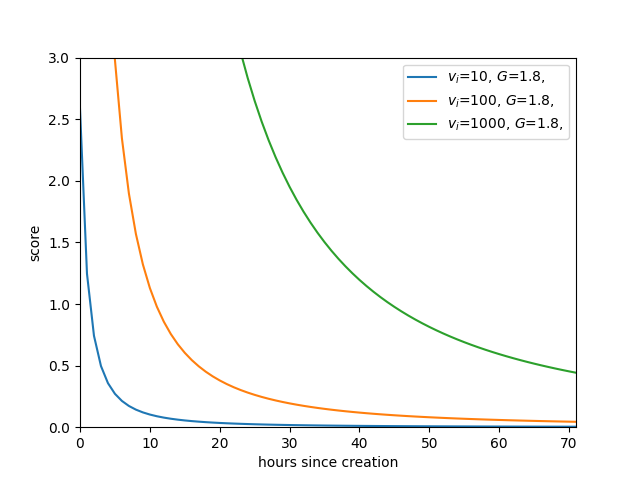
\includegraphics[width=\textwidth]{images/time_ranking_1.png}
    \caption{разное количество просмотров}
  \end{subfigure}
  \hfill
  \begin{subfigure}[b]{0.5\textwidth}
    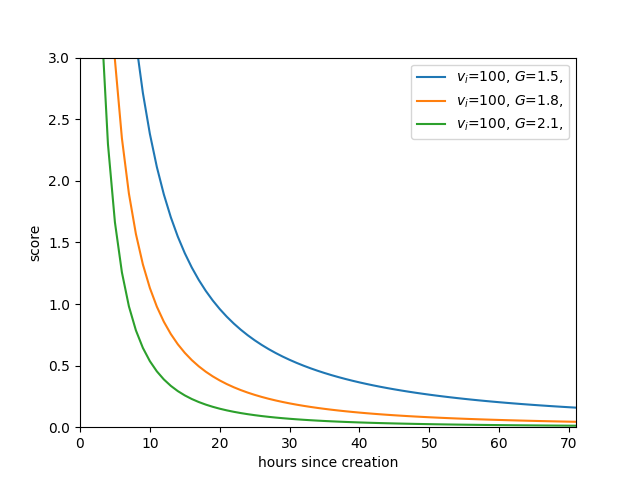
\includegraphics[width=\textwidth]{images/time_ranking_2.png}
    \caption{разный фактор гравитации}
  \end{subfigure}
\caption{ранжирование по времени}
    \label{fig:samples}
\end{figure}


В конце значиния нормализуются с помощью \texttt{min-max} нормализации.


\subsubsection{Фильтрация на основе категорий}
\label{content}

Мы представляем каждую новость как вектор значений достоверности (насколько сильно каждая новость относится к категории).

\begin{table}[h]
    \centering
    \begin{tabular}{cccccc}
        \toprule
        item\_id & \textit{politics} & \textit{IT} & \textit{social\_media} & $\cdots$ & \textit{confilcts} \\
        \midrule
        1 & 0.55 & 0 & 0 & $\cdots$ & 0.3 \\
        2 & 0    & 0.81  & 0.62 & $\cdots$ & 0 \\
        \vdots & \vdots & \vdots & \vdots & \vdots & \vdots\\

        \bottomrule
    \end{tabular}
    \caption{тексовые вектора}
    \label{tab:text_vectors}
\end{table}


Тегирование происходит следующим образом: составляем словарь принадлежности слов к категориям:

\begin{table}[h]
    \centering
    \begin{tabular}{cc}
        \toprule
        \textit{word} & \textit{category} \\
        \midrule
        trump & politics \\
        crash & accident \\
        telegeram & IT \\
        \vdots & \vdots \\
        \bottomrule
    \end{tabular}%
    \caption{категории слов}
    \label{tab:words_categories}
\end{table}

Уверенность берется из метрики слова tf-idf вместе со всем набором документов.

Количество слов ограничено, но в течение дня добавляются новые слова, а каждую ночь пересчитываются вектора элементов.

У нас есть действия, пока пользователь взаимодействует с системой, и веса для элементов для каждого взаимодействия (\cref {tab:action_score}).


\begin{table}[h]
    \centering
    \begin{tabular}{cc}
        \toprule
        \textit{action} & \textit{score} \\
        \midrule
        shown & -1 \\
        viewed & 2 \\
        emoji or comment & 1 \\
        read till the end & 1 \\
        \bottomrule
    \end{tabular}%
    \caption{веса взаимодействий}
    \label{tab:action_score}
\end{table}

Все данные агрегированы, и каждая новость имеет оценку действия в зависимости от того, что с ней сделал пользователь. Предположим, что пользователь просмотрел и оставил смайлик. Общий балл составит: $ -1 $ (пользователю был показан элемент) $ + 2 $ (пользователь просмотрел элемент) $ + 1 $ (пользователь оставил смайлик) $ = 2 $.

По мере взаимодействия пользователя с системой мы формируем его вектор предпочтений следующим образом:

\begin{equation}
    u_i = \sum_{j=1}^{n} v_j \times s_j
\end{equation}

\begin{itemize}
    \item $u_i$ -- вектор $user_i$
    \item $v_j$ -- вектор $item_j$
    \item $s_j$ -- вес взаимодействия с $item_j$
\end{itemize}

Пользовательский вектор имеет такую же размерность, что и вектор элемента.

Поскольку теперь у нас есть векторы пользователей и элементов, мы можем найти между ними сходство:


\begin{equation}
    r_{ui}=\cos (\theta)=\frac{\mathbf{u} \cdot \mathbf{v}}{\|\mathbf{u}\|\|\mathbf{v}\|}=\frac{\sum_{i=1}^{n} u_{i} v_{i}}{\sqrt{\sum_{i=1}^{n} u_{i}^{2}} \sqrt{\sum_{i=1}^{n} v_{i}^{2}}}
\end{equation}

\begin{itemize}
    \item $r_{ui}$ -- рейтинг $user$ $item$
    \item $u$ -- вектор $user$
    \item $v$ -- вектор $item$
\end{itemize}


Как было сказано ранее, фильтрация на основе содержимого имеет свой собственный вес воздействия, который вначале невелик (мы не хотим ограничивать доступ пользователя к контенту только потому, что он сделал несколько случайных щелчков), но он увеличивается по мере взаимодействия пользователя с системой и мы можем делать прогнозы относительно его категориальных предпочтений.


\subsection{Обзор компонентов ранжирования}


\subsubsection{Коллаборативная фильтрация}

Мы используем алгоритм SVD ++.

Для рекомендаций по коллаборативной фильтрации у нас должна быть матрица пользовательских оценок, которая формируется из истории оценок.

Мы используем модификацию Funk MF, которая факторизует матрицу рейтингов «пользователь-элемент» как произведение двух матриц меньшей размерности, первая имеет строку для каждого пользователя, а вторая имеет столбец для каждого элемента. Строка или столбец, связанные с конкретным пользователем или элементом, называются скрытыми признаками.

\begin{equation}
    r_{u i}=\sum_{f=0}^{n } H_{u, f} W_{f, i}
\end{equation}


Хотя Funk MF может обеспечить очень хорошее качество рекомендаций, но его способность использовать только явные числовые рейтинги в качестве взаимодействий между пользователями и элементами представляет собой ограничение. Современные рекомендательные системы должны использовать все доступные взаимодействия, как явные (например, числовые рейтинги), так и неявные (например, лайки, покупки, пропущенные, добавленные в закладки). С этой целью SVD ++ также был разработан с учетом неявных взаимодействий. По сравнению с Funk MF, SVD ++ также учитывает предвзятость пользователя и элемента.

Прогнозируемый рейтинг, который пользователь $ u $ поставит элементу $ i $, вычисляется следующим образом:

\begin{equation}
    r_{u i}=\mu+b_{i}+b_{u}+\sum_{f=0}^{n} H_{u, f} W_{f, i}
\end{equation}



\subsubsection{Фильтрация по популярности}

Для измерения популярности мы аггрегируем следующие данные: \hyperref[tab:show]{показы}, \hyperref[tab:view]{просмотры}, \hyperref[tab:emotion]{emoji}, \hyperref[tab:comment]{комментарии}.

\begin{table}[h]
    \centering
    % \resizebox{\textwidth}{!}{
    \begin{tabular}{ccccc}
        \toprule

        \emph{item\_id} & \emph{shows\_num} & \emph{views\_num} & \emph{emotions\_num} & \emph{comments\_num} \\\midrule

        1 & 1043 & 231 & 52 & 7  \\
        2 & 828  & 478 & 78 & 11 \\
        3 & 163  & 25  & 5  & 0  \\
        \vdots & \vdots & \vdots & \vdots & \vdots \\\bottomrule


     \hline
    \end{tabular}
    % }

    \caption{популярность элементов}
    \label{tab:popularity}
\end{table}

Таким образом, когда мы применяем информацию о популярности новостных статей, мы можем выставлять им оценки по следующему алгоритму:

\texttt{min-max} нормализуем \emph{shows\_num}, \emph{views\_num}, \emph{emotions\_num}, \emph{comments\_num}, затем делим на 4 (чтобы получить 1 как максимум после суммы) и суммируем все эти значения.

\begin{equation}
    r_i = \frac{\emph{shows\_num}}{4} + \frac{\emph{views\_num}}{4} + \frac{\emph{emotions\_num}}{4} + \frac{\emph{comments\_num}}{4} 
\end{equation}


\subsubsection{Фильтрация на основе содежимого (LDA)}

Для фильтрации на основе содержимого мы должны каким-то образом векторизовать новости и представлять предпочтения пользователей через эти векторизованные новости. Мы будем использовать латентное распределение Дирихле (LDA), которое представляет собой генеративную статистическую модель, которая позволяет объяснять наборы наблюдений группами, которые объясняют, почему некоторые части данных похожи. Например, если наблюдения представляют собой слова, собранные в тексты, предполагается, что каждый документ представляет собой смесь небольшого количества тем и что присутствие каждого слова связано с одной из тем документа.

Таким образом, мы можем векторизовать текст в зависимости от того, как каждый текст относится к каждой категории, от 0 до 1.
Например, предположим, что у нас есть 3 темы, извлеченные с помощью модели LDA:

\begin{table}[h]
\centering
% \resizebox{\textwidth}{!}{%
\begin{tabular}{ccc}
    \toprule
\textit{topic} & \textit{word} & \textit{score} \\
    \midrule
1 & dollar & 0.3 \\
1 & bank & 0.2 \\
1 & money & 0.15 \\
2 & sugar & 0.4 \\
2 & cooking & 0.3 \\
3 & IT & 0.25 \\
3 & hacker & 0.2 \\
\bottomrule
\end{tabular}%
% }
\caption{темы слов}
\label{tab:words_topics}
\end{table}

Допустим у нас текст: ``Hackers use mobile emulators to steal millions of dollars''. Его векторизованной формой будет $[0.3, 0, 0.2]$.

Все вычисления проведены в соостветствии с \ref{content}.


\subsubsection{Фильтрация на основе текущей сессии}

Мы хотим мгновенно реагировать на действия пользователя, поэтому применяем фильтрацию на основе текущей сессии следующим образом:
пытаемся найти новости, похожие на те, которые пользователь только что смотрел.

\begin{equation}
    r_{i}=\sum_{k=0}^{n} \textit{similarity}\{\textit{current\_item\_vector}, \textit{last\_viewed\_vector}_{k}\} \times \textit{weight}_k
\end{equation}


где $\textit{weight}_k$ это вес последней просмотренной новости. Вес тем больше, чем недавнее была просмотрена новость.



\subsection{Гибридная система}

Таким образом, наличие всей этой информации позволяет нам настраивать вклад каждой отдельной системы с помощью поиска по сетке. Таким образом, мы оптимизируем веса, которые влияют на каждую рекомендацию. Конкретные оптимизируемые метрики будут указаны ниже.
    




% \section{Implementation}
% \label{sec:implementation}

\section{Оценка качества}
\label{sec:evaluation}

\subsection{Обзор}

Для оценки у нас есть информация о том, какой список рекомендаций был дан каждому пользователю и каков источник рекомендации:

    \begin{table}[h]
        \centering
        \resizebox{\textwidth}{!}{  
        \begin{tabular}{cccc}
            \toprule
            \textit{user\_id} & \textit{recommendation\_list}       & \textit{content\_based\_filtering}  & \textit{collaborative\_filtering} \\
            \midrule
            2 & \{(2, 0.91), (1, 0.74), (3, 0.23)\} & \{(2, 0.45), (1, 0.54), (3, 0.08)\} & \{(2, 0.92), (1, 0.4), (3, 0.3)\}\\

            1 & \{(3, 0.73), (1, 0.69), (2, 0.15)\} & \{(2, 0.6), (1, 0.44), (3, 0.04)\} & \{(2, 0.58), (1, 0.58), (3, 0.14)\}\\
            \vdots & \vdots & \vdots & \vdots \\
            \bottomrule
        \end{tabular}%
        }
        
        \caption{логи выдачи рекомендаций}
        \label{tab:recommendation_logs}
    \end{table}

    \begin{itemize}
        \item \textit{recommendation\_list}: список рекомендаций, который состоит из пар (\textit{item\_id}, \textit{score})
        \item \textit{content\_based\_filtering \& collaborative\_filtering}: источники рекомендаций
    \end{itemize}

  Поскольку мы используем взвешенную сумму наших рекомендаций, у нас есть уникальные значения весов для каждого пользователя:

    \begin{table}[h]
        \centering
        \begin{tabular}{ccc}
            \toprule
            \textit{user\_id} & \textit{content\_based\_filtering} & \textit{collaborative\_filtering} \\
            \midrule
            1                 & 0.25                                  & 1                               \\
            2                 & 1                               & 0.5                                \\
            \vdots & \vdots & \vdots \\
            \bottomrule
            \end{tabular}%
        \caption{значения весов}
        \label{tab:boost_values}
    \end{table}

Чтобы проиллюстрировать подсчет оценок рекомендаций, взгляните на 1-ю строку таблицы \hyperref [tab:advice_logs] {журналы рекомендаций}. Мы видим рекомендацию $ r = \{(2, 0.91), (1, 0.74), (3, 0.23) \} $ для пользователя $ u = 2 $, поэтому мы должны найти значения повышения для этого конкретного пользователя в таблице \hyperref [tab:boost_values] {boost values}: усиление контентной фильтрации $ b_{cbf} $ для $ u $ составляет $ 1 $, усиление совместной фильтрации $ b_{cf} $ составляет $ 0,5 $. Итоговая оценка рассчитывается следующим образом: $ 0,91 = 0,45 * b_{cbf} + 0,92 * b_{cf} = 0,45 * 1 + 0,92 * 0,5 = 0,45 + 0,46 $.

    Также у нас есть информация о \hyperref [tab:show] {shows} и \hyperref [tab:view] {views}, поэтому мы можем отслеживать, какой элемент в списке рекомендаций был нажат, а какой элемент был пропущен, поэтому в зависимости от этого информация, которую мы можем отслеживать, понравился ли элемент пользователю или нет. Например, рассмотрим ситуацию, когда пользователь щелкнул 4-ю рекомендацию из списка рекомендаций. Это означает, что первые 3 рекомендации плохие, и мы должны штрафовать алгоритмы, которые отдавали приоритет этим элементам, учитывая тот факт, что 1-й элемент является худшим:


\begin{equation}
    \textit{penalty} = \frac{1}{\textit{num\_of\_item\_in\_rank}}
\end{equation}



% \subsection{Online}

% \subsection{Offline}

% \section{Further research}
% \label{sec:further}

\section{Итоги}
\label{sec:summary}


Система рекомендаций получила широкое распространение в разных сферах. Коллаборативная фильтрация фокусируется на рейтинге, игнорируя особенности самих элементов. Чтобы лучше оценивать предпочтения клиентов в отношении новостей, мы используем модель LDA для рассчёта предпочтения клиентов по новостным темам.

Чтобы прогнозировать рейтинг по новостям, мы принимаем во внимание схожесть клиентов и корреляцию между покупателями и новостями. Эксперимент показывает, что наш гибридный метод рекомендаций, основанный на характеристиках, лучше работает в нашем приложении для социальных сетей.

Мы предлагаем новый гибридный метод рекомендаций, основанный на функциях повышения качества выдачи.

Результаты показывают, что сочетание разных подходов приводит к увеличению вовлеченности пользователей. До внедрения рекомендательной системы пользователь тратил на вкладку новостей около 2 минут. Теперь, когда мы применили гибридную рекомендательную систему, пользователи проводят на вкладке новостей в среднем 5 минут.



\setmonofont[Mapping=tex-text]{CMU Typewriter Text}
\bibliographystyle{ugost2008ls}
\bibliography{diploma.bib}
\end{document}
